\part{Organizacja i bezpieczeństwo pracy}
\chapter{Prawa i obowiązki kierownika pociągu wynikające z regulaminu pracy}
Prawa pracownika to w szczególności:
\begin{itemize}
	\item zatrudnienie na stanowisku pracy zgodnie z umową o pracę i posiadanymi kwalifikacjami,
	\item terminowe wynagrodzenie za pracę, 
	\item odpoczynek w dniach wolnych od pracy oraz po zakończeniu pracy, 
	\item płatny urlop wypoczynkowy, 
	\item jednakowe i równe traktowanie przez pracodawcę z tytułu wypełniania jednakowych obowiązków, 
	\item wykonywanie pracy w warunkach zgodnych z zasadami bezpieczeństwa i higieny pracy.
\end{itemize}
Do obowiązków pracownika należą w szczególności:
\marginnote{Regulamin pracy, rozdział III, \S 6-12}

\begin{itemize}
	\item rzetelne i efektywne wykonywanie pracy,
	\item przestrzeganie czasu pracy i wykorzystanie go w sposób jak najbardziej efektywny, w pełni na pracę zawodową,
	\item podporządkowanie się poleceniom pracowników usuwających awarię, lub prowadzących akcję ratowniczą, czy ewakuację,
	\item dbałość o dobro i mienie pracodawcy oraz zachowywanie w tajemnicy informacji technicznych, technologicznych, handlowych lub organizacyjnych, tajemnicy przedsiębiorstwa,
	\item przestrzegania zasad współżycia społecznego.
\end{itemize}
     Pracownik zobowiązany jest zapobiegać wszystkiemu, co zagraża bezpieczeństwu ruchu kolejowego, bezpieczeństwu ludzi oraz bezpieczeństwu mienia pracodawcy. 

\chapter{Obowiązki kierownika pociągu z jedno- i wieloosobową obsadą konduktorską}

Do zadań kierownika pociągu podczas pracy, należy:
\begin{enumerate}
	\item przyjmowanie i zdawanie składu pociągu,
	\item prowadzenie na bieżąco dokumentacji pociągowej,
	\item organizowanie pracy podległej drużyny konduktorskiej
	\item nadzorowanie podległych pracowników drużyny konduktorskiej tj. konduktorów, pracowników odbywających szkolenie praktyczne i innych
	pracowników wykonujących pracę w pociągu,
	\item kontrola dokumentów przewozu i odprawa podróżnych oraz udzielanie informacji w sprawach taryfowych i rozkładu jazdy pociągów KSL,
	\item Zapewnienie podróżnym niezbędnej pomocy podczas wsiadania i wysiadania z pociągu, w tym w szczególności osobom niepełnosprawnym i osobom
	o ograniczonych zdolnościach ruchowych,
	\item zgłaszanie na stacjach początkowych gotowość pociągu do odjazdu,
	\item nadzór nad odjazdem pociągu z miejsca wyznaczonego postoju do czasu, gdy nie opuści on peronów,
	\item stały kontakt z maszynistą, a w razie potrzeby zatrzymanie pociągu,
	\item rozstrzyganie sporów pomiędzy obsługą pociągu i podróżnymi oraz pomiędzy współpodróżnymi, o ile spór pomiędzy współpodróżnymi utrudnia podróż innym osobom,
	\item wykonywanie poleceń pracowników posterunków technicznych zarządcy	infrastruktury, organów kontrolnych i zwierzchnich, mających związek
	z wykonywaną pracą. Kierownik pociągu ma prawo odmówić wykonania polecenia lub też wstrzymać jego wykonanie, jeśli wykonanie wiązałoby się ze
	stworzeniem sytuacji zagrażającej bezpieczeństwu ruchu kolejowego. Ma on w takich przypadkach również prawo uchylić takie polecenie, wydane
	podległym pracownikom,
	\item wykonywanie w razie potrzeby pracy manewrowej,
	\item nadzór nad przestrzeganiem przepisów porządkowych i stanem bezpieczeństwa w pociągu,
	\item udzielanie pierwszej pomocy w nagłych wypadkach przed przybyciem lekarza lub pogotowia,
	\item wykonywanie wymaganej próby hamulca i oględzin technicznych w przypadku braku rewidenta,
	\item w razie potrzeby sprzęganie i rozprzęganie elektrycznych zespołów trakcyjnych, jeżeli posiada stosowne uprawnienia,
	\item ustalenie długości, masy ogólnej pociągu, rzeczywistej i wymaganej masy hamującej, obliczenie największej dozwolonej prędkości jazdy pociągu (gdy rzeczywista masa hamująca jest mniejsza od wymaganej masy hamującej),
	\item bieżący nadzór nad stanem technicznym urządzeń taboru, w tym także nad działaniem SIP i rzetelnością informacji tam wyświetlanych oraz rzetelnością innych informacji zamieszczanych przez spółkę wewnątrz pojazdów,
	\item w razie potrzeby zabezpieczanie taboru przed zbiegnięciem,
	\item wdrażanie procedur postępowania w razie zaistnienia wypadku, incydentu lub wydarzenia,
	\item informowanie dyżurnego ruchu o wszelkich zauważonych nieprawidłowościach,
	\item informowanie dyspozytora Spółki i sporządzenie raportu o wszelkich zaistniałych w trakcie zmiany roboczej nieprawidłowościach.
	\item Obsługa urządzeń głośnomówiących i podawanie komunikatów dla pasażerów w standardach przyjętych przez spółkę,
	\item Informowanie podróżnych o wszelkich kwestiach związanych z przejazdem, w tym o możliwościach skomunikowania z innymi przewoźnikami kolejowymi.
\end{enumerate}
Kierownik pociągu jest pracownikiem odpowiedzialnym za obsługiwany pociąg na wyznaczonym odcinku obsługi. Kierownikowi pociągu podlegają wszyscy
pracownicy obsługujący pociąg, za wyjątkiem organów nadzoru i kontroli.

\section{Obsada pociągu}
\label{sec:obsada}
Obsadę pociągu stanowi drużyna pociągowa, w skład której wchodzi drużyna trakcyjna oraz drużyna konduktorska lub tylko drużyna trakcyjna. Jednoosobowa drużyna trakcyjna dopuszczalna jest w pociągach kursujących z prędkościami nieprzekraczającymi 130km/h \marginnote{Instrukcja K-4, \S.2, pkt.3 - zwróć uwagę poniżej}, o ile pojazd jest wyposażony w sprawne urządzenia kontrolujące czujność prowadzącego pojazd kolejowy, lub w pociągu wyposażonym w urządzenia ERTMS/ETCS poziomu 1 lub 2 na liniach kolejowych wyposażonych w urządzenia tego systemu. \marginnote{Rozporządzenie Ministra Infrastruktury z dnia 20 października 2023 r. zmieniające rozporządzenie w sprawie ogólnych warunków prowadzenia ruchu kolejowego i sygnalizacji (Dz.U.2023.2474), dopuszcza do 160km/h przy jednoosobowej drużynie trakcyjnej}

Pociągi pasażerskie przewożące pasażerów powinny mieć obsadę konduktorską składającą się co najmniej z kierownika pociągu. Pociągi pasażerskie mogą jeździć bez kierownika pociągu jeżeli zamykanie drzwi pojazdu kolejowego przy wymianie podróżnych jest zapewnione, a zamknięcie drzwi jest sygnalizowane kierującemu pojazdem kolejowym z napędem za pomocą urządzeń technicznych. 

W przypadkach uszkodzenia urządzeń CA/SHP lub urządzeń radiołączności, przy jednoosobowej obsłudze trakcyjnej, kierownik pociągu powinien zająć miejsce w kabinie sterowniczej. W przypadku braku kierownika pociągu prowadzący pojazd kolejowy ma obowiązek doprowadzić pociąg do najbliższej stacji i postępować zgodnie z przepisami wewnętrznymi przewoźnika. 

\section{Znajomość typu pojazdu kolejowego}

Kierownik pociągu przed zatrudnieniem po raz pierwszy na stanowisku kierownika, na pociągu zestawionym z nowego typu pojazdu kolejowego, winien uzyskać znajomość typu pojazdu kolejowego. Znajomość typu pojazdu kolejowego utrzymuje się przez sześć miesięcy od czasu ostatniej jazdy w charakterze kierownika. Kierownikowi pociągu \textbf{nie wolno} wykonywać obowiązków w pociągu zestawionym z taboru dla którego nie posiada aktualnej znajomości typu pojazdu kolejowego. 

\section{Znajomość linii kolejowych}

Prowadzący pojazd kolejowy lub pociąg oraz kierownik pociągu powinni znać obsługiwane odcinki linii kolejowych, na których prowadzą pociąg. Kierownik pociągu i konduktor powinien również posiadać znajomość warunków techniczno - eksploatacyjnych stacji znajdujących się na tych odcinkach. 

Jeżeli maszynista nie posiada znajomości odcinków linii na których ma prowadzić pociąg, może go prowadzić, pod warunkiem że podczas jazdy obok niego znajduje się inny maszynista lub pracownik ZLK posiadający udokumentowaną znajomość tych
odcinków (pilot). W przypadku jeśli nie ma pilota, prowadzący pojazd powinien jechać ostrożnie, nie przekraczając prędkości 40km/h. W tym przypadku prowadzącemu pojazd kolejowy lub pociąg należy wydać rozkaz pisemny „O” informujący o okolicznościach mających wpływ na bezpieczeństwo jazdy pociągu, których znajomość jest konieczna do prowadzenia pojazdu kolejowego lub pociągu na tym odcinku.

Jeżeli kierownik pociągu otrzyma polecenie jazdy na odcinku, którego warunków obsługi nie zna, powinien o tym powiadomić pracownika, który wydał mu takie polecenie, a następnie zastosować się do jego dalszych poleceń. Kierownik pociągu nie znający obsługiwanych odcinków linii kolejowych w wyjątkowych przypadkach może obsługiwać pociąg kursujący na tych odcinkach, o ile zapozna się dokładnie z dotyczącymi danymi, zawartymi w wewnętrznym rozkładzie jazdy pociągów i dodatkach do niego. O nieznajomości obsługiwanych odcinków linii kolejowych przez kierownika pociągu należy ustnie powiadomić prowadzącego pojazd kolejowy tego pociągu.

\subsection{Dokumentowanie znajomości odcinków linii}

Zasady dokumentowania uregulowane są w Uchwale Zarządu 271/2017 z 07.11.2017 dot. znajomości odcinków linii kolejowych i taboru.

Do dokumentowania znajomości odcinków linii kolejowych służą:
\begin{enumerate}
	\item Karta znajomości odcinków/linii kolejowych
	\item Wykaz nabywania znajomości odcinków linii kolejowych oraz jazd w czynnej kabinie maszynisty
\end{enumerate}


\section{Przyjęcie pociągu na stacji początkowej}
Przyjęcie pociągu i przygotowanie go do drogi na stacji początkowej i torach
postojowych przez kierownika pociągu polega na:
\begin{itemize}
	\item spisaniu pojazdów kolejowych i sporządzeniu „wykazu pojazdów kolejowych w składzie pociągu”, obliczeniu, na podstawie danych z wykazu pojazdów kolejowych w składzie pociągu, masy brutto, masy hamującej, wymaganej i rzeczywistej, ilości wagonów, długości pociągu i innych niezbędnych danych,
	\item sprawdzeniu stanu technicznego przyjmowanego składu pod względem bezpieczeństwa ruchu kolejowego i podróżnych,
	\item sprawdzeniu działania toalet, stanu czystości pojazdów oraz uzupełnienia zbiorników wodnych, stan zbiorników fekalii, zaopatrzenia w materiały eksploatacyjne, w tym materiały sanitarne (mydło, papier toaletowy, ręczniki i inne materiały, jeśli są wymagane),
	\item sprawdzeniu lub dokonaniu prawidłowego \textbf{zewnętrznego i wewnętrznego oznakowania} składu pociągu tablicami kierunkowymi i numeracyjnymi,
	prawidłowości działania elektronicznych \textbf{tablic relacyjnych} oraz weryfikacja	stanu ilościowego i technicznego tablic malaturowych,
	\item dopilnowaniu lub dokonaniu przepisowego \textbf{osygnalizowania pociągu},
	\item dopilnowaniu lub wykonaniu \textbf{oględzin technicznych pociągu} na stacjach, na których nie ma rewidentów taboru,
	\item dopilnowaniu lub wykonaniu właściwej \textbf{próby hamulca pociągu}.
\end{itemize}

W przypadku wieloosobowej drużyny konduktorskiej kierownik pociągu następujące czynności może zlecić konduktorowi:
\begin{itemize}
	\item sprawdzenie słyszalności sygnału ostrzegawczego dla pasażerów, czytelności napisów ostrzegawczych oraz sprawność działania lokalnego
	(indywidualnego) otwierania drzwi przez pasażerów,
	\item sprawdzenie wyposażenia zespołu trakcyjnego, autobusu szynowego lub wagonów pod względem zgodności z inwentarzem,
	\item odnotowanie stwierdzonych braków wyposażenia ewidencyjnego zespołu trakcyjnego lub wagonu w Książce pokładowej pojazdu trakcyjnego lub w
	Książce pokładowej wagonu,
	\item sprawdzenie stanu technicznego sprzętu p.poż., urządzeń ogrzewczych, wentylacji i klimatyzacji,
	\item sprawdzenie prawidłowości działania automatycznego zamykania oraz blokady drzwi wejściowych pojazdów,
	\item sprawdzenie, czy wszystkie nie używane sprzęgi powietrzne są podwieszone na wspornikach,
\end{itemize}

Kierownik pociągu może odmówić przyjęcia składu pociągu wyłącznie wtedy, gdy stwierdzi, że znajdujący się w nim tabor zagraża bezpieczeństwu ruchu lub podróżnych. Odmowę przyjęcia składu wraz z podaniem przyczyny, kierownik pociągu niezwłocznie zgłasza do Dyspozytury Spółki oraz odnotowuje w:
Wykazie pojazdów kolejowych, Książce pokładowej pojazdu trakcyjnego lub w Książce pokładowej wagonu, dokonując stosownego potwierdzenia podpisem
i pieczątką identyfikacyjną.

\begin{tcolorbox}
	\begin{enumerate}
		\item Czy kierownik pociągu może odmówić przyjęcia składu pociągu?
		\begin{enumerate}
			\item Nie, decyzję podejmuje rewident na podstawie oględzin technicznych,
			\item Nie, decyzję podejmuje dyspozytor taborowy,
			\item Tak, jeżeli skład pociągu zagraża bezpieczeństwu ruchu kolejowego i podróżnym.
		\end{enumerate}
		\item Czy kierownik pociągu może przebywać w kabinie maszynisty podczas jazdy pociągu?
		\begin{enumerate}
			\item Nigdy
			\item Jeżeli zostanie wezwany przez maszynistę w określonych przypadkach,
			\item Jeżeli takie polecenie otrzyma od dyspozytora.
		\end{enumerate}
	\end{enumerate}
\end{tcolorbox}

\chapter{Prowadzenie dokumentacji pociągowej}

Zgodnie z rozporządzeniem Ministra Transportu, w pociągu powinny znajdować się następujące dokumenty:
\begin{enumerate}
	\item dopuszczenie do użytkowania lub przywrócenie do eksploatacji
	\item karta próby hamulca i urządzeń pneumatycznych, zwana dalej „kartą próby hamulca”;
	\item wykaz pojazdów kolejowych w składzie pociągu;
	\item książka pokładowa wagonu – w wagonie pasażerskim i typu pasażerskiego.
\end{enumerate}

Dopuszczenie do użytkowania, oraz karta próby hamulca powinny znajdować się w czynnej kabinie maszynisty, zaś wykaz pojazdów w składzie pociągu u kierownika pociągu.

\section{Dopuszczenie do użytkowania lub przywrócenie do eksploatacji}
Dokument ten zgodnie z przepisami przyjętymi w Spółce znajduje się wewnątrz ksiązki pokładowej zespołu trakcyjnego. Wskazuje on kto i kiedy dopuścił pojazd do eksploatacji po dokonaniu czynności utrzymaniowych i naprawczych. Dokument ten wskazuje również wszelkie ograniczenia w eksploatacji, nałożone przez ECM (Spółkę) lub instytucje zewnętrzne.
\marginnote{Instrukcja K-1, \S.19-20}

\section{Karta próby hamulca i urządzeń pneumatycznych}
Przy próbie kartę próby hamulca należy wypełnić w sposób następujący:
Na stronie pierwszej kierownik pociągu lub pracownik upoważniony wypełnia następujące rubryki:
\begin{itemize}
	\item „nazwa stacji” wpisuje nazwę stacji na której wykonano próbę, wpisuje datę, imię, nazwisko i podpis wystawiającego,
	\item w pozycji 1 należy wpisać „S” dla próby szczegółowej, „U” dla próby uproszczonej,
	\item na podstawie dokumentów pociągowych i rozkładu jazdy kierownik pociągu wypełnia:
	\begin{itemize}
		\item (poz.2) Numer pociągu
		\item (poz.3) Miejsce wykonywania próby (stacja lub posterunek)
		\item (poz.4) Data i godzina \textbf{zakończenia} próby
		\item (poz.8 oraz 9) Masa ogólna składu (M\textsubscript{os}) i masa ogólna pociągu (M\textsubscript{o}) (zasady wyliczania \ref{def:masa})
		\item (poz.11) Masa hamująca rzeczywista M\textsubscript{hr}
		\item (poz. 12) Procent masy hamującej wymaganej P\textsubscript{w} - zobacz ilustrację \ref{fig:pw})
	\end{itemize}
	\item (poz. 5,6,7) na podstawie zgłoszenia osoby wykonującej próbę hamulca  wpisuje numer inwentarzowy pojazdu trakcyjnego lub kabiny/członu
	\item kierownik pociągu dokonuje obliczeń:
		\begin{itemize}
			\item (poz. 10) Masy hamującej wymaganej M\textsubscript{hw} (wzór \ref{wzr:mhw})
			\item (poz.13) Procent masy hamującej rzeczywistej P\textsubscript{r}(wzór \ref{def:pr})
		\end{itemize}
	\item (poz. 14 i 15) na podstawie wskazań manometrów w tylnej kabinie maszynisty wpisanie ciśnienia (wyłącznie po wykonywaniu próby szczegółowej, w przypadku próby uproszczonej wykreślamy te pola)
	\item po sprawdzeniu sprawności urządzeń sterowania hamulcem ep, hamulca elektrodynamicznego, urządzeń sterowania drzwiami wejściowymi, oraz innych urządzeń, takich jak toaleta w systemie zamkniętym, drzwi przejściowe, wpisuje w pola 16 - 19 słowa TAK lub NIE.
	\item w polach 20 i 21 wpisuje dwa pierwsze pojazdy za lokomotywą (lub licząc od czoła EZT) oraz dwa ostatnie pojazdy (wagony)
	\item w polu 22 wpisuje numer pojazdu z nieczynnym hamulcem umieszczonego na końcu składu.	
\end{itemize}

Na stronie nr 2 kierownik pociągu lub pracownik upoważniony wypełnia: „informację o układzie hamulcowym w składzie pociągu” w następujący sposób:
\begin{itemize}
	\item opisać stan hamulców w wagonach znakami w ten sposób, że: koniec pociągu należy oznaczyć symbolem „]”,
	pojazdy z wyłączonym hamulcem zespolonym należy oznaczyć symbolem „X”, 
	pojazdy z czynnym hamulcem ręcznym należy oznaczyć symbolem „O”.
	\item kierunek wyjazdu ze stacji pośrednich należy oznaczyć „O” zakreślając strzałkę, oraz wpisać nazwę stacji, nieczynne urządzenia zamykania drzwi w pojeździe przeznaczonym do 	przewozu osób oznaczyć symbolem „N”.
	\item wpisać numery inwentarzowe (EVN) wagonów z nieczynnym hamulcem.
\end{itemize}

W polu \textbf{podpis prowadzącego próbę} składa osoba która dokonywała sprawdzenia zahamowania i odhamowania (przy próbie uproszczonej na pojazdach z hamulcem tarczowym jest to maszynista pociągu, w pozostałych przypadkach kierownik pociągu lub rewident). 

Jeśli wykonywana była \textbf{próba szczegółowa} dla połączonego składu dwóch lub więcej EZT, należy założyć karty próby dla każdego EZT, pamiętając o poprawnym wypełnieniu informacji o numerze pojazdu z którego czynnej kabiny próbę wykonywano. Jeśli wykonywana była \textbf{próba uproszczona} dla takiego składu, wypełniamy jedynie jedną kartę próby - wyłącznie dla tego EZT z którego czynnej kabiny wykonano próbę.

\section{Wykaz pojazdów kolejowych w składzie pociągu}
W wykazie pojazdów kolejowych w składzie pociągu, zamieszcza się następujące dane:

\begin{itemize}
\item identyfikatory pojazdów kolejowych włączonych do składu pociągu;
\item długości poszczególnych pojazdów kolejowych i ich długość łączną;
\item masę poszczególnych pojazdów kolejowych (netto, tarę i brutto) i ich masę łączną;
\item masę hamującą rzeczywistą poszczególnych pojazdów kolejowych i ich łączną rzeczywistą masę hamującą;
\item stację nadania i stację przeznaczenia wraz z numerami węzłów kolejowych;
\item ewentualne informacje o przewożonych towarach niebezpiecznych wraz z numerem klasyfikacyjnym wynikającym z regulaminu RID.
\end{itemize}

Wzór wykazu pojazdów w składzie pociągu jest drukiem wstępnie wypełnionym. Należy uzupełnić pola dotyczące obsady drużyny pociągowej i odcinka obsługiwanego, typ i numer serii pojazdu, numery EVN, oraz długość pojazdu, masę netto pojazdu, masę ładunku oraz masę hamującą rzeczywistą. Następnie należy te wartości przepisać do pola H1, lub zsumować w polach H2 i H3 w przypadku jazdy ukrotnionej.

W przypadku wykazu wypełnianego na ''druku zgodnym z rozporządzeniem''\marginnote{Rozporządzenie Ministra Transportu z dnia 2 listopada 2006 r. w sprawie dokumentów, które powinny znajdować się w pojeździe kolejowym, Dz.U.2007.9.63} w górnej części formularza wprowadzamy informację o obsadzie drużyny pociągowej, jako jednostkę macierzystą należy wprowadzić identyfikator literowy przewoźnika.

W kolumnie 3, w pole państwo rejestracji wpisujemy \textbf{PL}, w kolumnie 4 wpisujemy \textbf{KSL}, dla spółki nie nadano cyfrowego identyfikatora eksploatującego pojazd kolejowy (kol. 6). Kolumny 11,12 oraz 14 należy wykreślić (przewożenie materiałów niebezpiecznych w składzie pociągu pasażerskiego jest zabronione). W kolumnie 13, przekreślić opis w nagłówku i wpisać \textbf{brutto} - a następnie w tej kolumnie wpisać masę brutto pociągu. Pozostałe pola w tej części tabeli wypełniamy zgodnie z informacjami zamieszczonymi na pudle EZT lub wagonów (masa własna pojazdu, masa ładunku, długość pojazdu, masa hamująca rzeczywista). Należy również zsumować te dane do wiersza H1 - H6.
W wierszu H1 - H6 wpisujemy parametry pociągu w następującej kolejności: Masa ogólna składu M\textsubscript{os}, Masa ogólna pociągu M\textsubscript{o}, Masa hamująca wymagana M\textsubscript{hw}, Masa hamująca rzeczywista M\textsubscript{hr}, Procent m.h. wymaganej P\textsubscript{w}, Procent m.h. rzeczywistej P\textsubscript{r}. Koniecznie pamiętaj o wpisywaniu jednostek miary (tony i procenty).

\section{Książka pokładowa wagonu}
Książka pokładowa wagonu służy do:
\begin{itemize}
\item przekazywania przez drużynę konduktorską obsłudze technicznej informacji o uszkodzeniach stwierdzonych w wagonie w czasie jego jazdy;
\item zapisu stwierdzonych przez obsługę techniczną uszkodzeń i wykonanych czynności naprawczych w wagonie w czasie postoju na stacji postojowej lub przyczyn wyłączenia wagonu z ruchu;
\item powiadamiania eksploatującego wagon o stwierdzonych uszkodzeniach, wykonanych czynnościach naprawczych lub przyczynach wyłączenia wagonu z ruchu.
\end{itemize}
Książka składa się z:
\begin{enumerate}
\item formularza meldunkowego (w kolorze białym), który wypełnia drużyna konduktorska w czasie jazdy pociągu albo obsługa techniczna na stacji \item formularza warsztatowego (w kolorze żółtym), w którym wpisy uzupełniają pracownicy obsługi technicznej na stanowiskach naprawczych;
\item formularza własnego wagonu (w kolorze różowym), który, po wykonaniu prac naprawczych lub zabezpieczających, przekazuje się z wagonem eksploatującemu pojazd kolejowy.
\end{enumerate}

\section{Książka pokładowa pojazdu z napędem}

Książka pokładowa pojazdu z napędem składa się z trzech części z których w pierwszej odnotowuje się stan urządzeń związanych z bezpieczeństwem (radiotelefon, czuwak aktywny, shp) oraz przebieg pojazdu. W części drugiej dokonuje się wpisów dotyczących dokonywanych czynności przeglądowych, oględzin technicznych, prób hamulca i wyposażenia. W części trzeciej odnotowuje się przeglądy i roboty naprawcze. W części trzeciej odnotowuje się usterki i czynności naprawcze.

\chapter{Użytkowanie urządzeń radiołączności pociągowej}

\marginnote{Instrukcja K-7, Rozdział II}

Radiołączność pociągowa służy do zapewnienia łączności pomiędzy:
\begin{enumerate}
\item dyżurnym ruchu i maszynistą pojazdu trakcyjnego znajdującego się na przyległym szlaku,
\item dyżurnymi ruchu sąsiednich posterunków - w przypadku wystąpienia całkowitej przerwy w łączności przewodowej, maszynistami pojazdów trakcyjnych znajdujących się na tym samym szlaku,
\item obchodowymi służby drogowej, eksploatacji i maszynistą pojazdu trakcyjnego jadącego po danym szlaku lub między obchodowymi i dyżurnymi
ruchu posterunków ograniczających dany szlak - wyłącznie w przypadkach zagrożenia bezpieczeństwa ruchu,
\item obsługą stanowisk kontroli urządzeń do wykrywania w czasie jazdy stanów awaryjnych taboru i maszynistami pojazdów trakcyjnych,
\item kierownikiem pociągu i maszynistą pojazdu trakcyjnego prowadzącego dany pociąg.
\item dróżnikiem przejazdowym i maszynistą w zakresie odbioru i wysyłania sygnału RADIO-STOP
\end{enumerate}

Dla sieci radiołączności pociągowej na poszczególnych liniach kolejowych przydzielone są odpowiednie kanały pracy. Przy przejeździe z jednej linii na drugą należy przełączyć radiotelefon na kanał obowiązujący na danej linii.

Numery kanałów obowiązujących na poszczególnych liniach kolejowych zarządcy infrastruktury podane są w zeszytach wewnętrznego rozkładu jazdy
pociągów i oznaczone literą ,,R'' z dodaniem cyfry oznaczającej numer kanału od 1 do 7. np.,,R6'', a punkty zmiany kanału na linii określone są wskaźnikami W28, zobacz na ilustracji \ref{fig:w28}.

Drużyna konduktorska może nawiązywać łączność z \textbf{prowadzącym pojazd kolejowy} z napędem w celu:
\begin{itemize}
	\item wymiany informacji
	\item konieczności wezwania do najbliższej stacji pomocy (policja, pogotowie itp.),
	\item podania sygnału „Gotów do odjazdu" (w zespołach trakcyjnych i wagonach silnikowych). W tym celu należy postępować zgodnie
	z zasadami podanymi w § 7.
\end{itemize}
\marginnote{Instrukcja Ir-5, \S.11, ust.3}
W przypadku zagrożenia bezpieczeństwa ruchu lub potrzeby \textbf{skomunikowania pociągów} pasażerskich drużyna konduktorska może nawiązać łączność bezpośrednio z \textbf{dyżurnym ruchu}. 

W przypadku korzystania z radiotelefonu przewoźnego aby nawiązać łączność z dyżurnym ruchu, należy wykorzystać przyciski wywołania/blokady szumu ZEW3. W przypadku łączności z innym pociągiem należy użyć przycisku ZEW1. 

W przypadku zaistnienia nagłego zagrożenia bezpieczeństwa ruchu, bezpieczeństwa podróżnych na linii wyposażonej w radiotelefoniczną łączność
pociągową, należy zastosować alarmowe zatrzymanie ruchu pociągów przez nadanie sygnału ,,ALARM'' za pomocą radiotelefonu. Prócz podania sygnału
,,ALARM'' należy podjąć działania zapobiegające wypadkowi lub zmniejszające ich skutek.

Sygnał ,,ALARM'' może być nadany w sposób:
1) automatyczny,
2) słowny - gdy w radiotelefonie nie ma przycisku ,,ALARM''.

Automatyczne nadanie sygnału ,,ALARM'' uzyskuje się przez wciśnięcie i przytrzymanie przez około 10 sekund w manipulatorze przycisku oznaczonego
napisem ,,ALARM''. Spowoduje to włączenie nadajnika i cykliczne samoczynne wysyłanie sygnału alarmowego. Sygnał ten jest odbierany przez odbiorniki
wszystkich urządzeń pracujących aktualnie na tym kanale i znajdujących się w zasięgu radiotelefonu emitującego ,,ALARM'' w postaci kombinacji trzech tonów słyszanych w głośnikach urządzeń odbierających oraz urządzenia nadającego. Powoduje to natychmiastowe samoczynne zahamowanie wszystkich pociągów znajdujących się w zasięgu i wyposażonych w urządzenia systemu „Radio-Stop”, których radiotelefony odebrały sygnał ,,ALARM''. Skasowanie sygnału ,,ALARM'' należy przeprowadzić w sposób określony w instrukcji obsługi danego typu radiotelefonu. 

Odebranie sygnału ,,ALARM'' nadanego automatycznie zobowiązuje wszystkich użytkowników, którzy go odebrali do przełączenia radiotelefonu
na kanał ratunkowy (kanał nr 8 w radiotelefonach przewoźnych, kanał nr 2 w radiotelefonach stacjonarnych) w celu wyjaśnienia przyczyny nadania
tego sygnału z najbliższym dyżurnym ruchu.

W celu nadania sygnału ,,ALARM'' słownie należy wypowiedzieć do mikrofonu co najmniej pięć razy słowo ,,ALARM''.
Pracownicy, którzy usłyszeli w swoich radiotelefonach sygnał "ALARM” nadany \textbf{słownie} powinni natychmiast przerwać prowadzone rozmowy.
Wyjaśnienie przyczyn jego nadania dokonuje się na kanale, \textbf{na którym nadany został} ten sygnał.

Prowadzący pojazdy kolejowe z napędem i pracownicy wyposażeni w radiotelefony przenośne, po usłyszeniu sygnału ,,ALARM'' zobowiązani są
natychmiast zatrzymać pojazd kolejowy, o ile nie nastąpiło to już samoczynnie.

Istnieją również sieci radiołączności stacyjnej, oraz liniowej - drogowej, SOK, zasilania elektroenergetycznego, ratunkowa. W kanał sieci ratunkowej R-8 wyposażone są wszystkie radiotelefony posiadające kanały pociągowe.



\chapter{Podawanie i odbieranie sygnałów kolejowych w zakresie drużyny pociągowej}

Przed odjazdem pociągu z miejsca, w którym wyznaczono postój dla wsiadania i wysiadania podróżnych po upewnieniu się, że nie ma przeszkód do
odjazdu drużyna konduktorska podczas procedury odjazdu pociągu wykorzystuje następujące sygnały:
\begin{itemize}
	\item Rp 11 „Wsiadać” – podawany przed odjazdem pociągów pasażerskich,
	\item Rp 12 „Gotów do odjazdu” - stosuje się przed odjazdem pociągów
	z wieloosobową drużyną konduktorską,
	\item  Rp 13 „Pociąg nr..... gotów do odjazdu” - sygnał ten kierownik pociągu przekazuje słownie lub za pomocą urządzeń łączności do maszynisty; stosuje 	się go przed odjazdem pociągów zestawionych z \textbf{elektrycznych zespołów trakcyjnych} i pojazdów silnikowych (autobusów szynowych) w przypadku, gdy urządzenia do sterowania drzwiami i sygnałem dźwiękowym ostrzegającym
	podróżnych znajdują się \textbf{na pulpicie w kabinie maszynisty}, lub zamykanie	drzwi pojazdu kolejowego przy wymianie podróżnych jest zapewnione,	a zamknięcie drzwi pojazdu kolejowego jest przekazywane kierującemu	pojazdem kolejowym z napędem za pomocą urządzeń technicznych,
	\item Rp 14 „Odjazd pociągów pasażerskich” – w pociągach wyposażonych w sterowane przez kierownika pociągu urządzenia sygnałowe do dawania
	sygnału „Odjazd”; sygnał ten podaje się za pomocą tych urządzeń.
\end{itemize}

Kierownik pociągu podaje w kierunku konduktorów sygnał Rp 12, drużyna konduktorska podaje sygnał Rp 11, po upewnieniu się, że nie ma przeszkód do odjazdu pociągu, konduktorzy podają kolejno od najdalszego konduktora w kierunku kierownika pociągu sygnał Rp 12, po otrzymaniu sygnału Rp 12 od najbliższego konduktora, kierownik pociągu podaje: w kierunku maszynisty sygnał \textbf{Rp 14} na pociągach złożonych z \textbf{lokomotywy i wagonów pasażerskich}, a jeżeli kierownik pociągu znajduje się w końcu lub środku pociągu, to sygnał Rp 14 podany przez kierownika pociągu konduktorzy powtarzają kolejno w kierunku maszynisty, albo sygnał \textbf{Rp 13} na pociągach złożonych z \textbf{zespołów trakcyjnych},

\chapter{Postępowanie w razie zagrożenia bezpieczeństwa podróżnych}
Do czasu podjęcia akcji przez jednostki specjalistyczne, kierującym wszystkimi działaniami na pokładzie pojazdu jest kierownik pociągu przy ścisłej współpracy wszystkich członków personelu pokładowego. 
W celu zapewnienia możliwości identyfikacji Kierownika pociągu na miejscu zdarzenia powinien on nosić kompletne umundurowanie (jeżeli jest to możliwe założyć kamizelkę ostrzegawczą). 
W przypadku nieobecności kierownika pociągu, kierownictwo obejmuje maszynista pociągu, który ma obowiązek realizować wszystkie obowiązki Kierownika pociągu.
Zapamiętać możliwie najwięcej szczegółów odnośnie podejrzanego przedmiotu, zjawiska czy osoby/osób w celu przekazania wyczerpującego meldunku służbom ratowniczym,
W celu uniknięcia paniki w pojeździe telefoniczny meldunek o zagrożeniu należy złożyć w kabinie maszynisty w obecności maszynisty.

Na podstawie oceny zagrożenia Kierownik Pociągu wspólnie z Dyżurnym Ruchu podejmuje decyzję w zakresie sposobu dalszego postępowania. W przypadku zarządzenia ewakuacji pociągu następuje ona w lokalizacji wskazanej przez Kierownika Pociągu.
Jeżeli Kierownik pociągu uzna, że decyzje Dyżurnego ruchu w zakresie dalszego trybu postępowania są nieadekwatne do sytuacji lub stan zagrożenia wymaga podjęcia niezwłocznych działań np. ewakuacji pasażerów Kierownik pociągu przeprowadza ewakuację w wybranej przez siebie lokalizacji i informuje o tym Dyżurnego Ruchu.

Komunikat o ewakuacji pociągu przekazuje Kierownik Pociągu za pośrednictwem urządzeń
nagłaśniających lub (w przypadku braku takich urządzeń na pojeździe kolejowym) słownie - przechodząc przez skład pociągu.
Komunikat dla pasażerów winien zawierać polecenie oddalenia się od miejsca zagrożenia
względnie (jeśli pozwalają na to warunki miejscowe) ukrycia się za budynkami lub innymi obiektami w celu zminimalizowania narażenia pasażerów na skutki potencjalnego niebezpieczeństwa. Kierownik pociągu ma obowiązek sprawdzenia czy wszyscy pasażerowie opuścili skład pociągu.
\marginnote{Art. 15. ustawy Prawo Przewozowe
	\begin{enumerate}
	\item 	Podróżny jest obowiązany do przestrzegania przepisów
	porządkowych obowiązujących w transporcie.
	\item Osoby zagrażające bezpieczeństwu lub porządkowi w transporcie mogą być
	niedopuszczone do przewozu lub usunięte ze środka transportowego.
	\item Osoby uciążliwe dla podróżnych lub odmawiające zapłacenia należności za
	przewóz mogą być usunięte ze środka transportowego, chyba że naruszałoby to zasady współżycia społecznego.
	\end{enumerate}
}

Każdorazowo interwencja policji realizowana jest \textbf{na wniosek} kierownika pociągu. Podstawą do usunięcia podróżnego z pociągu jest Ustawa Prawo Przewozowe (art. 15.1) oraz Rozporządzenie Ministra Infrastruktury z dnia 23 listopada 2004 r. w sprawie przepisów porządkowych obowiązujących na obszarze kolejowym, w pociągach i innych pojazdach kolejowych z późniejszymi zmianami, w którym określone są zakazy obowiązujące na terenie kolejowym. 


\chapter{Postępowanie w razie zagrożenia bezpieczeństwa ruchu kolejowego}

\section{Cofanie, dzielenie i zabieranie częściami składu pociągu ze szlaku}

\ \ Bez pozwolenia dyżurnego ruchu nie jest dozwolone cofanie pociągu z wyjątkiem nagle grożącego niebezpieczeństwa. Po
uzgodnieniu z dyżurnym ruchu posterunku zapowiadawczego, w kierunku którego pociąg ma cofać, na pierwszym wagonie w
kierunku cofania powinien znajdować pracownik celem obserwacji toru szlakowego i zahamowania pociągu w razie potrzeby.
Drużyna trakcyjna powinna cofać pociąg ze szczególną ostrożnością, nie przekraczając prędkości 30km/h a 20 km/h przez
przejazdy kolejowo-drogowe i przejścia, które nie są obsługiwane lub zabezpieczone w inny sposób.

\ \ W przypadku nagłego niebezpieczeństwa, cofanie pociągu ze szlaku bez uzgodnienia z dyżurnym ruchu należy wykonać z
prędkością najwyżej 5 km/h, pod warunkiem że w odległości drogi hamowania pociąg będzie poprzedzał właściwy pracownik z
przyborami sygnałowymi i że widoczność nie jest mniejsza niż 100m.

Bezwzględnie nie wolno cofać pociągu jeśli:

\begin{enumerate}
\item Pociąg jedzie bez drużyny konduktorskiej
\item Na szlaku z wieloodstępową (samoczynną) blokadą liniową, jeśli nie otrzymano pozwolenia dyżurnego ruchu
\item W czasie gdy widoczność jest mniejsza niż 100m, a nie uzgodniono z dyżurnym ruchu
\item jeżeli pociąg jedzie na jednotorowym odcinki linii kolejowej bez obsady stacji i mijanek i bez urządzeń sterowania
zdalnego, jeśli nie otrzymano pozwolenia dyżurnego ruchu odcinkowego.
\end{enumerate}
Cofany pociąg należy zatrzymać na 100 m przed semaforem odstępowym jeśli nie podawany jest sygnał do mnie, przed
urządzeniem sygnałowym ważnym dla cofanego pociągu, obok semafora wjazdowego znajdującego się przy sąsiednim torze z
prawej strony w kierunku cofania, lub w odległości 100 m przed pierwszym rozjazdem na drodze cofanego pociągu.

Jeżeli po zatrzymaniu pociągu drużyna stwierdzi że część pociągu może dalej jechać, należy powiadomić dyżurnych ruchu tylnego ( w pierwszej kolejności) i przedniego posterunku zapowiadawczego. Po otrzymaniu wiadomości o podzieleniu lub rozerwaniu pociągu na szlaku dyżurny ruchu zamyka tor szlakowy. Pozostającą na szlaku część pociągu należy zahamować i jeżeli to możliwe, strzec.

Przed odjazdem części pociągu ze szlaku należy dla niej wykonać próbę hamulca. Na odjeżdżającej części pociągu nie można umieszczać sygnałów końca pociągu, należy zanotować numer ostatniego wagonu, aby sprawdzić czy ta część pociągu dojechała do stacji w całości.

O zbliżaniu się tylko części pociągu dyżurny ruchu powinien uprzedzić zainteresowanych nastawniczych (zwrotniczych), przede wszystkim zaś posterunek nastawniczego obsługującego semafor wjazdowy od strony tego szlaku, z którego zbliża
się część pociągu.

Wjazd na stację poszczególnych części pociągu następuje na zasadach podanych dla ruchu po torze zamkniętym.Po pozostałą na szlaku część pociągu należy wysłać lokomotywę z tą samą drużyną, która przyprowadziła na stację część pociągu i (o
ile jest to możliwe) wysłać również odpowiedniego pracownika do pomocy.

\section{Rozerwanie pociągu na szlaku i zbiegnięcie wagonów}

Po zatrzymaniu rozerwanego pociągu na szlaku należy hamulcem postojowym lub ręcznym zahamować w oderwanej części składu odpowiedni procent masy ogólnej. Po wykonaniu czynności wymienionych w ust. 1, jeżeli obsada pociągu na to pozwala, to należy przednią częścią rozerwanego pociągu dojechać do części oderwanej, a następnie obie części połączyć, wykonać próbę hamulca, wagony odhamować i jechać dalej. Gdy połączenia obu części pociągu nie można wykonać, należy niezwłocznie zawiadomić o tym dyżurnego ruchu tylnego posterunku ruchu i porozumieć się z nim co do sposobu zwolnienia toru szlakowego. Wagon z uszkodzonymi urządzeniami sprzęgowymi należy, o ile to jest możliwe, zabrać z pierwszą częścią pociągu, łącząc go z tą częścią nawet w sposób prowizoryczny.

W razie zbiegania wagonów ze stacji w kierunku szlaku, należy je wszelkimi sposobami zatrzymać, a gdy to jest niemożliwe, skierować na tor żeberkowy lub inny tor stacyjny, a gdy i to nie jest możliwe – wykoleić na wykolejnicy lub w inny sposób, np. za pomocą podkładania podkładów itp. 

Na szlaku z wieloodstępową (samoczynną) blokadą liniową nie należy cofać pociągu jadącego naprzeciw zbiegłych wagonów, lecz pociąg zatrzymać.

\chapter{Wykonanie zahamowania pociągu w kabinie maszynisty}

Przed rozpoczęciem jazdy kierownika pociągu w czynnej kabinie maszynisty - w sytuacjach określonych w rozdziale Obsada pociągu (\ref{sec:obsada}) - maszynista pojazdu powinien poinstruować o sposobach zatrzymania pojazdu, a także odpisać ten fakt w książce pojazdu trakcyjnego.

Zahamowanie pociągu w kabinie maszynisty można wykonać przy pomocy nastawnika hamowania (zaworu maszynisty), poprzez pociągnięcie tegoż nastawnika do oporu (do siebie). Istnieje również możliwość użycia przycisku awaryjnego, koloru czerwonego (tzw. grzybek) znajdującego się po obu stronach pulpitu maszynisty. W pojazdach typu EN75 (Stadler Flirt) na ściance bocznej po lewej stronie od fotela maszynisty znajduje się dźwignia awaryjnego hamowania. 

W pojeździe EN57 ze względu na brak przycisku awaryjnego, oraz budowę i lokalizację zaworu hamulcowego zahamowanie pojazdu należy wykonywać przy pomocy hamulca bezpieczeństwa znajdującego się na ścianie oddzielającej kabinę maszynisty od przedziału służbowego.
\begin{marginfigure}
	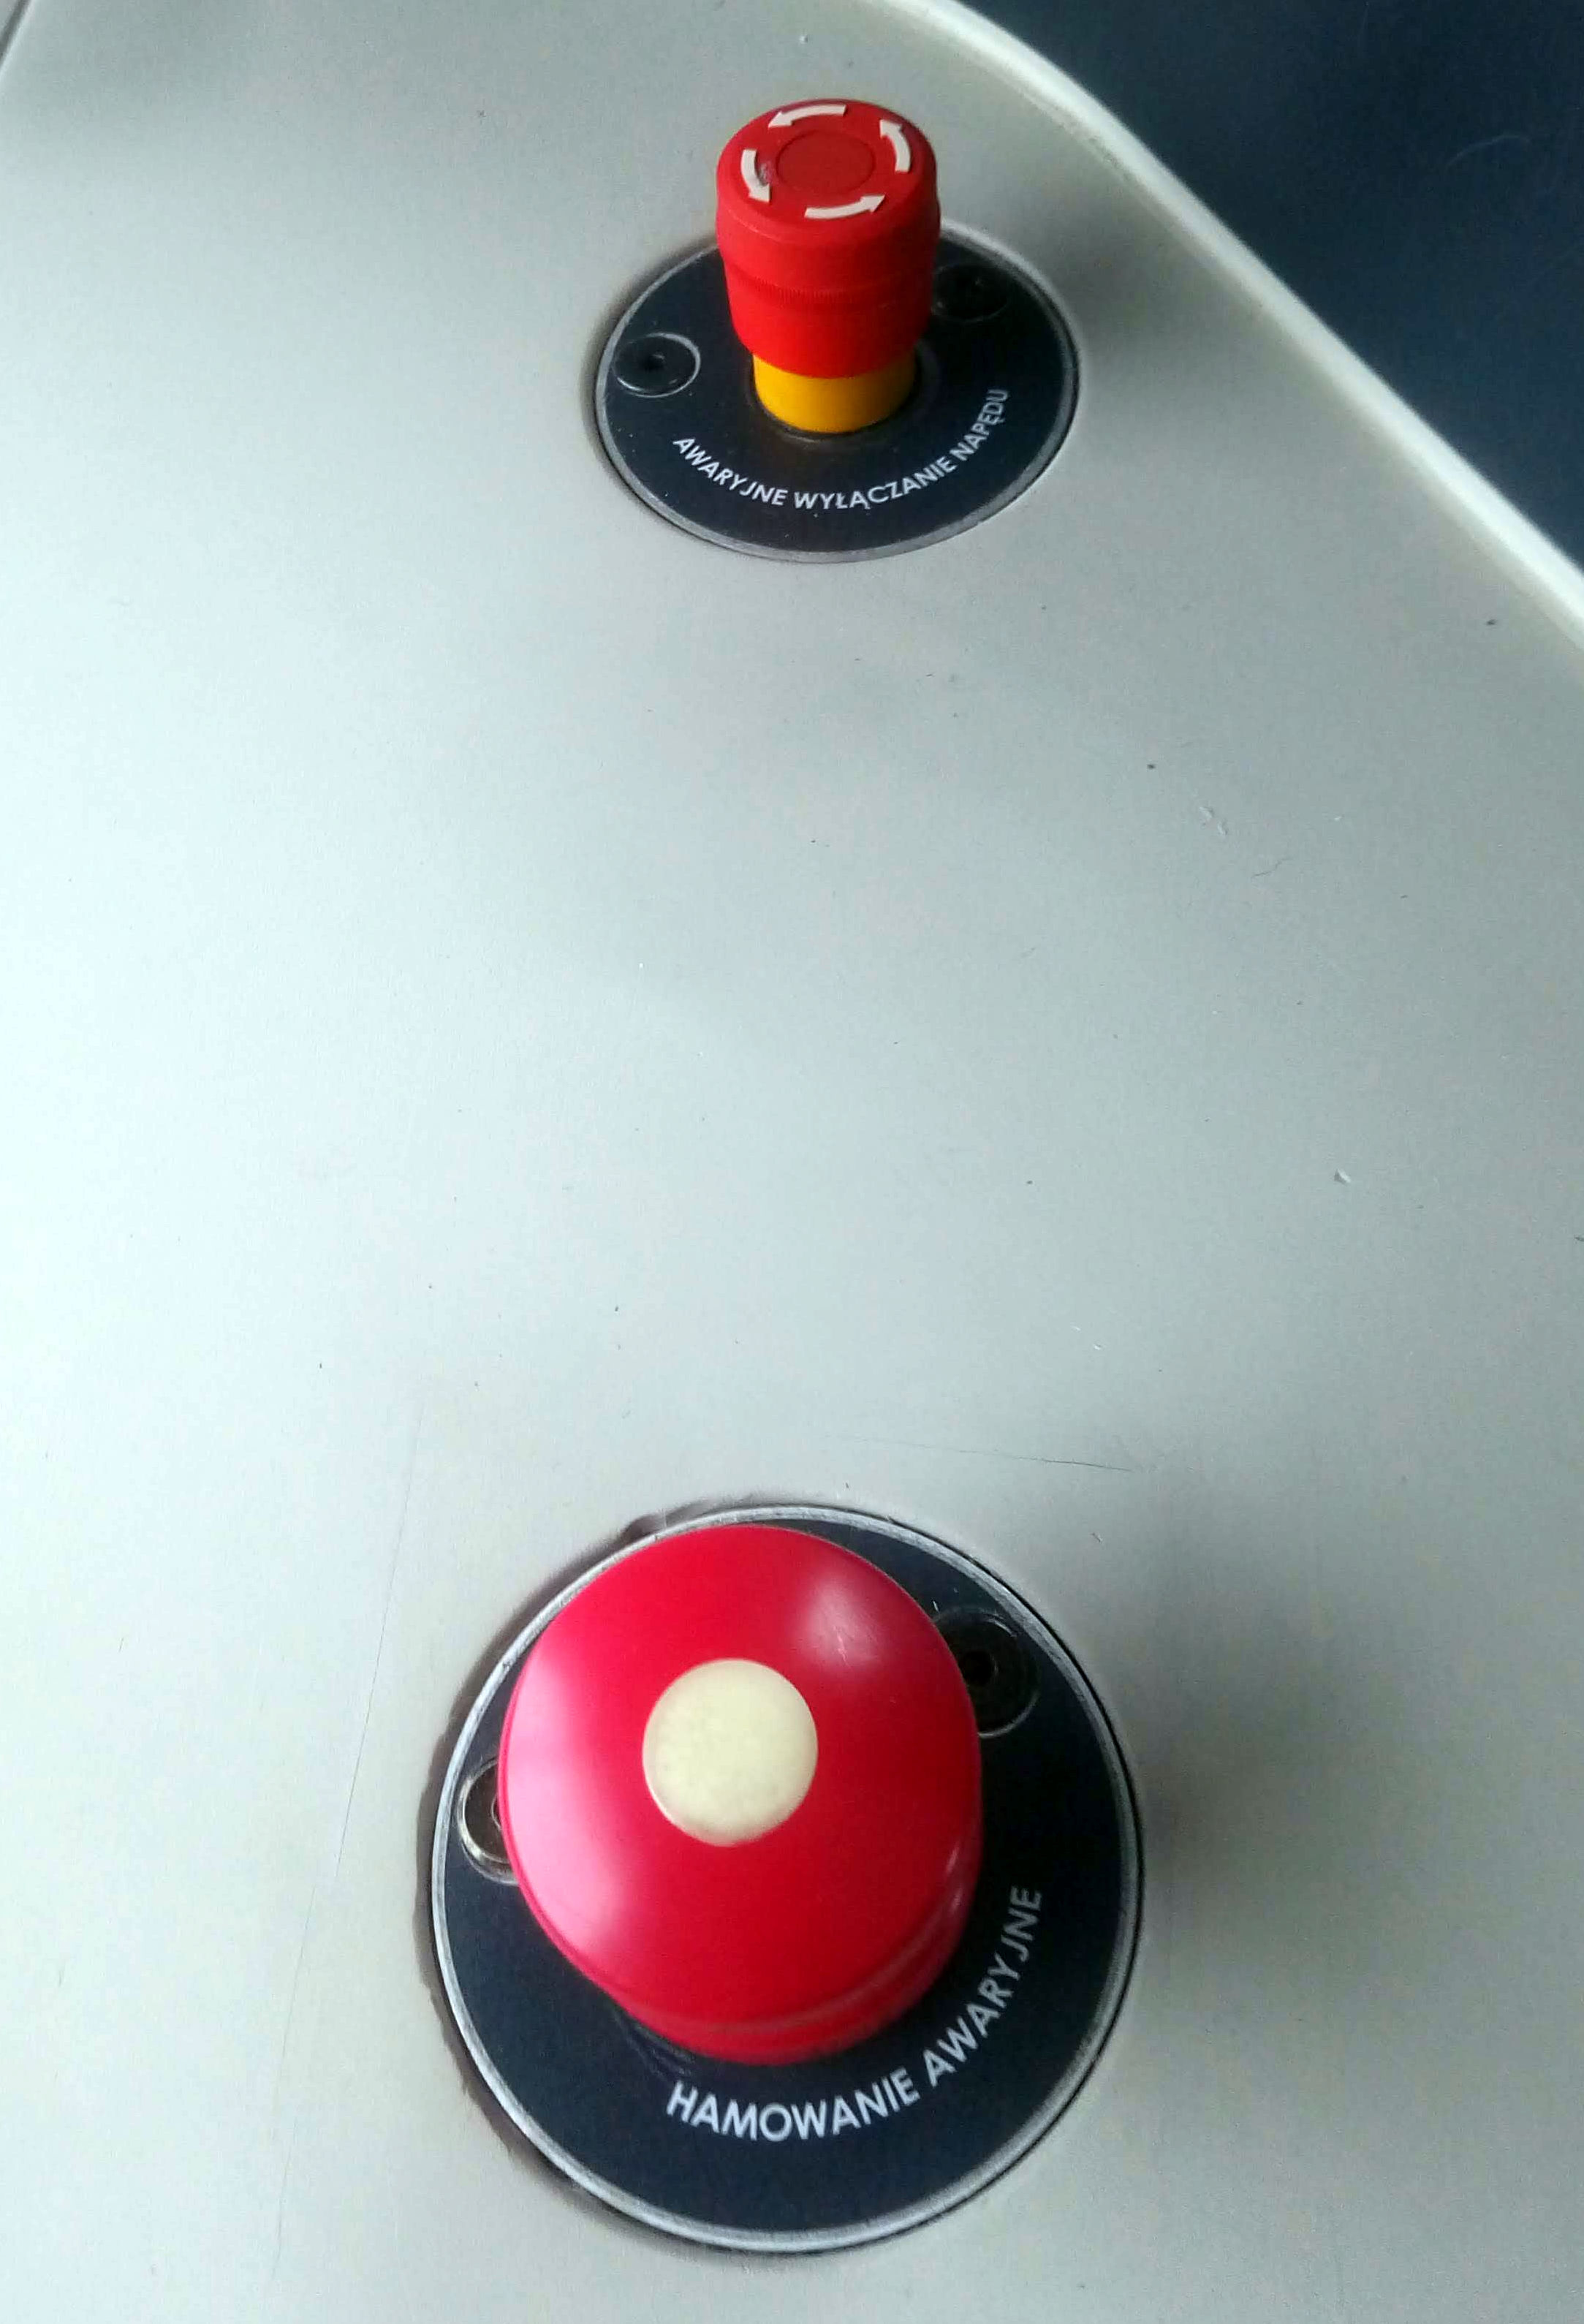
\includegraphics[width=5cm]{skryptkierownik-img/grzybek.jpg}
	\caption{Przyciski awaryjnego hamowania i awaryjnego wyłączania napędu w pojeździe EN76}
\end{marginfigure}


\chapter{Odłączanie urządzeń energetycznych pojazdu w nagłych przypadkach}

\begin{marginfigure}
	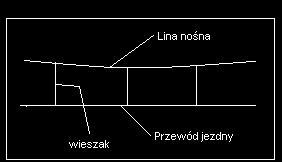
\includegraphics[width=5cm]{skryptkierownik-img/siec-jezdna.jpg}
	\caption{Elementy sieci trakcyjnej}
\end{marginfigure}
Na sieci kolejowej zarządzanej przez PKP PLK jak również częściowo na sieciach czeskiej i słowackiej, sieć trakcyjna zasilana jest napięciem 3kV prądu stałego (w praktyce ok. 2400-3600V). Najczęstsze uszkodzenia sieci trakcyjnej polegają na zerwaniu przewodu jezdnego, obniżeniu sieci trakcyjnej (np. po upadku na sieć drzewa, etc.), zerwaniu wieszaka lub wysięgnika i znajdowaniu się tych elementów poniżej przewodu jezdnego, co może doprowadzić do uszkodzenia pantografu.

Rezystancja ciała człowieka waha się w dość szerokich granicach (od kilkuset omów,, do kilkuset $k\Omega$). Składa się na nią rezystancja przejścia między urządzeniem a ciałem, rezystancja naskórka, rezystancja wewnętrzna organizmu. Przyjmuje się, że rezystancja ciała człowieka wynosi $1000\Omega$. Najgroźniejszymi z prądów rażeniowych są prądy o częstotliwościach 40 ÷ 60 Hz gdyż wywołują one migotanie komór sercowych. W związku z tym przyjmuje się że napięcia i natężenia uznawane za bezpieczne w przypadku prądu zmiennego mają o połowę niższą wartość.
\begin{marginfigure}
	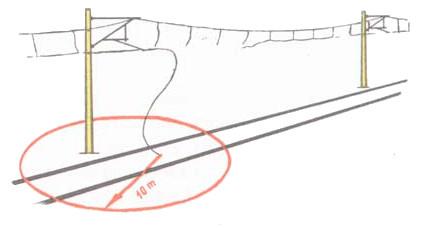
\includegraphics[width=5cm]{skryptkierownik-img/strefa-niebezpieczna-trakcja-10.jpg}
	\caption{Strefa niebezpieczna wokół zerwanego przewodu jezdnego}
	\label{fig:przewod}
\end{marginfigure}
W warunkach środowiskowych, w których rezystancja ciała człowieka wynosi co najmniej 1000 Ω, przyjmuje się że napięcia dzielimy w następujący sposób:
\begin{table*}
	\begin{tabular}{|c|m{2.5cm}|m{2.5cm}|}
		\hline
		Napięcie&Przemienne& Stałe\\
		\hline
		Bezpieczne &<25V &<50V\\
		\hline
		Warunkowo bezpieczne &25V-50V &50V-100V\\
		\hline
		Niebezpieczne	&>50V	&>100V\\
		\hline
	\end{tabular}
	\caption{Napięcia bezpieczne i niebezpieczne}
\end{table*}

Strefa niebezpieczna wokół zerwanego przewodu dotykającego ziemi, szyny, lub wiszącego nad torem wynosi \textbf{10m}. W tym obszarze poruszanie się wyłącznie nie odrywając jednej z nóg, lub odrywając równocześnie obie nogi (''\textit{skacząc jak żabka}''). Jeżeli przewód trakcyjny jest zerwany i dotyka pojazdu, a nie ma innych zagrożeń, takich jak pożar, nie powinniśmy w ogóle zezwalać na opuszczanie pojazdu przez podróżnych.

Odległość bezpieczna od urządzeń zasilających i sieci trakcyjnej pod napięciem wynosi \textbf{1,4m}.
\begin{marginfigure}
	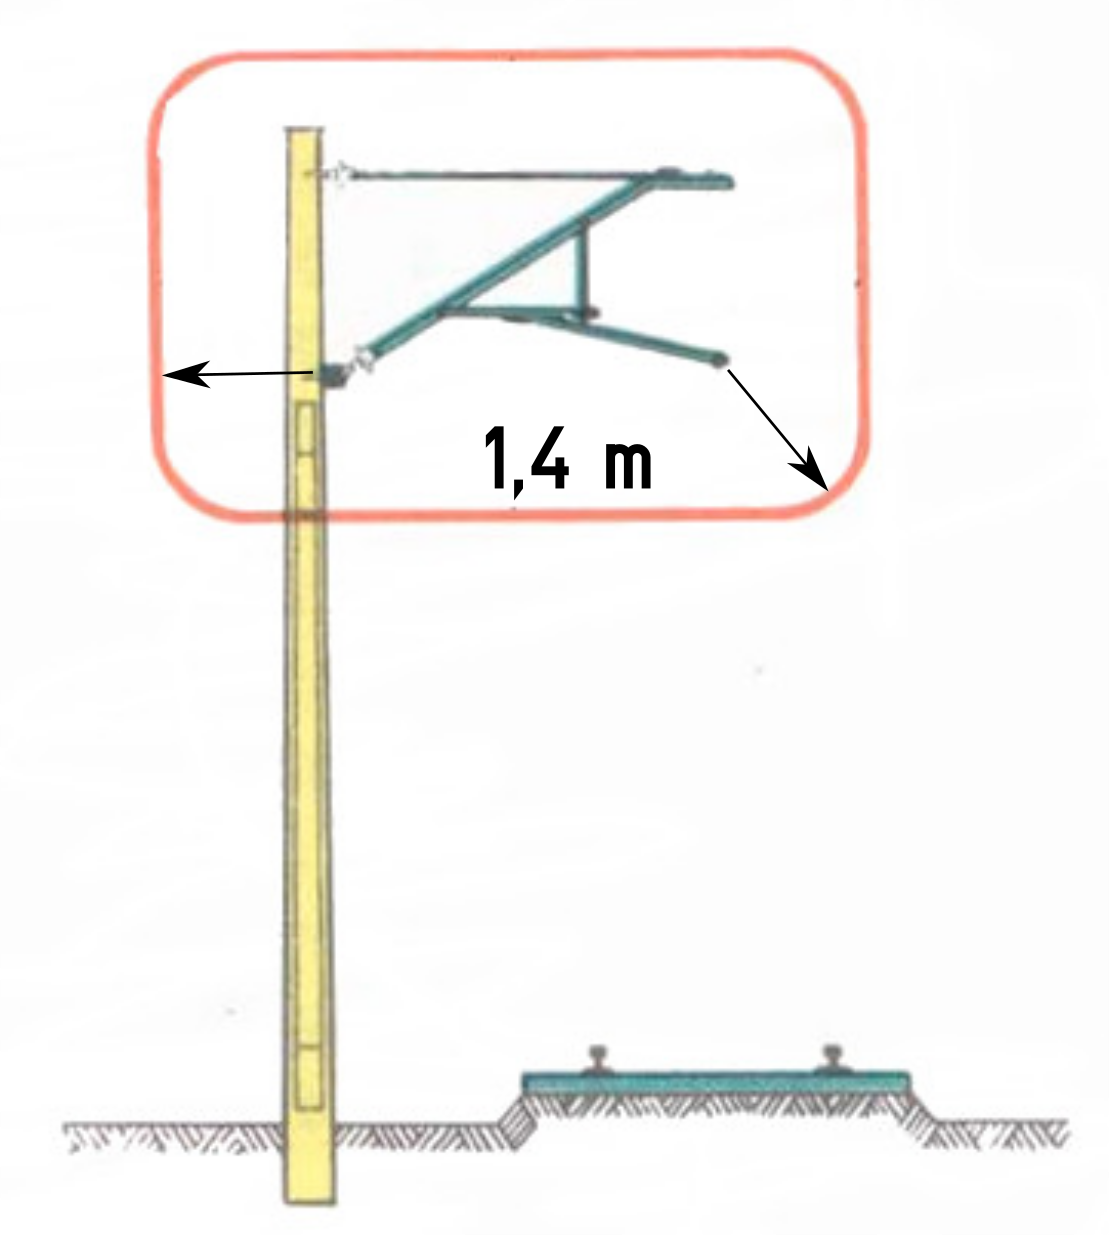
\includegraphics[width=5cm]{skryptkierownik-img/strefa-niebezpieczna-trakcja-14.png}
	\caption{Strefa niebezpieczna wokół urządzeń i przewodów sieci trakcyjnej}
	\label{fig:strefa}
\end{marginfigure}
Wszelkie prace wykonywane przy urządzeniach wysokiego napięcia takie jak uszynianie, muszą być prowadzone w asyście drugiej osoby. Kierownikowi pociągu nie wolno jednak wykonywać żadnych czynności przy urządzeniach elektroenergetycznych. Drużynie konduktorskiej nie wolno również rozpinać sprzęgu elektrycznego pomiędzy lokomotywą oraz wagonami (tą czynność może wykonywać maszynista pojazdu trakcyjnego).

Przy próbie ratowania człowieka porażonego przez prąd elektryczny, nie należy go dotykać gołymi rękoma, a jedynie probować odepchnąć (oderwać), przy pomocy drąga, lub kopnięciem. Następnie należy wyciągnąć go poza strefę niebezpieczną. Najczęściej osoba porażona przez prąd elektryczny znajduje się w stanie nagłego zatrzymania krążenia, oraz może posiadać głębokie oparzenia. Pierwsza pomoc takiej osobie polega na prowadzeniu resuscytacji krążeniowo-oddechowej, oraz w miarę możliwości użyciu AED.






